\documentclass{assignment}

\usepackage{fancyvrb}
\usepackage{url}
\usepackage{hyperref}
\usepackage{xcolor}


\mytitle{C4M: Human Mobility and Epidemic Modelling}

\begin{document}

\newcommand{\comment}[1]{{\color{blue} Comment: \color{blue}{#1}}}
\section*{Introduction and Overview}

Researchers use models of epidemics to predict whether and how an epidemic can be contained. Using models of epidemics to arrive at conclusions with public health implications has a long history. As far back as the 18th century, the Swiss mathematician and physicist Daniel Bernoulli modelled the spread of smallpox~\cite{Bernoulli}. 

Modelling an epidemic requires modelling the disease -- specifying to what extent it is infectious and how fast individuals can recover; and modelling human mobility -- specifying how far and how fast people can travel.  Once a model is built and validated, it can be used to predict outbreaks of various diseases using computer simulations.

For this project, you will be implementing an algorithm that illustrates the
spread of a disease through different cities. Given a list of cities 
and the times to travel between them, your program will first calculate the shortest time
from the initially infected city to every other city. Then you will simulate the spread of an epidemic through these cities.

In this project, you will be working on modelling human mobility using \href{https://en.wikipedia.org/wiki/Graph_(discrete_mathematics)}{graphs}. Although we will be using graphs to represent travel distance, graphs are useful in a variety of settings, such as bioinformatics and genomics. 

\vspace*{-0.5cm}
\section*{Part 1: Representing Travel Times Between Cities}

For Part 1, you will implement five helper functions and submit them on PCRS.  Before starting to implement the helper functions, finish reading the full description of Part 1. 

Your goal for Part 1 is to write functions that will help you read data about flights from a file and build a dictionary with information about direct flights between cities.  For example, consider the contents of file \verb|cities.txt| below, which represents data about a flight network shown in the picture on the right:

\vspace*{-0.3cm}
\begin{minipage}[c]{0.45\linewidth}
\begin{verbatim}
  Toronto:New York 3
  New York:Washington 2
  Washington:San Francisco 3
  San Francisco:Mexico City 3
  Toronto:Mexico City 7
  Toronto:San Francisco 6
\end{verbatim}
\end{minipage}
\hspace{1cm}
\begin{minipage}[c]{0.45\linewidth}
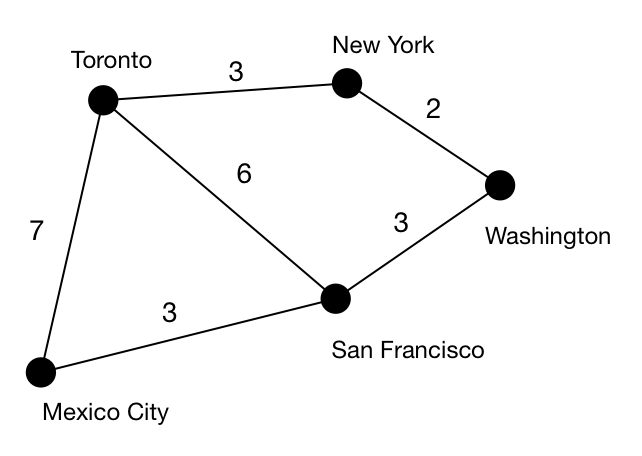
\includegraphics[width=6cm]{figs/map.png}
\end{minipage}
\vspace*{-0.5cm}

The data means, for example, that there is a 3-hour direct flight from Toronto to New York, {\bf and} a 3-hour direct flight from New York to Toronto. We say that Toronto and New York are neighbours. On the other hand, there is no direct flight from Toronto to Washington (or vice-versa), so they are not neighbours. 

For our program, we will store this direct-flight distance information in a dictionary where the keys will represent departure cities and the values
will be lists of tuples. Each tuple will have an arrival city and a duration. The dictionary that matches our example would look
like this: 
\begin{verbatim}
{'Toronto': [('Mexico City', 7), ('New York', 3), ('San Francisco', 6)],
'New York': [('Toronto', 3), ('Washington', 2)],
'Washington': [('New York', 2), ('San Francisco', 3)],
'San Francisco': [('Mexico City', 3), ('Toronto', 6), ('Washington', 3)],
'Mexico City': [('Toronto', 7), ('San Francisco', 3) ]}
\end{verbatim}

Notice that all 12 flights (the 6 original flights in the data and the 6 return flights) are stored in the dictionary.

\subsection*{Start Coding with Some Helper Functions}
On PCRS, in Part 1, you will find the following functions that you must implement.

\begin{tabular}{|l|p{10cm}|}
\hline
{\bf Name} & {\bf Basic Description} \\ \hline
\verb|get_closest(unvisited)| & \verb|unvisited| is a list of tuples of city name and distance. Return the tuple from this list for which the distance is smallest. \\ \hline
\verb|find_city(city, city_list)| & Return the index in \verb|city_list| of the first tuple that contains \verb|city|.  \\\hline
\verb|process_line(line)| & Return a tuple containing the information from a string of the format \verb|"first city name:second city name distance"|. \\ \hline
\verb|build_adjacent_distances(lines)| & From a list of lines (each of which are the format required as input to \verb|process_line|), return a dictionary that contains all the direct-flight distances between pairs of cities.\\ \hline
\verb|get_all_cities(city_to_city_dist)| & Return a sorted list of all the cities that appear in the distance dictionary \verb|city_to_city_dist|.\\ \hline


\end{tabular} 

This is only a basic description of each function. More details are given in the docstrings and the problem descriptions on PCRS.
Because the error messages in PCRS can be obscure, we recommend first writing your code in Wing. You may want to skip ahead to the next section and download the starter code so you can open it in Wing. If you do this, don't forget to copy your work back into PCRS to check the test cases and to submit it for credit.
\vspace*{-0.6cm}
\section*{Part 2: Finding the Shortest Time to Get to a City}

Your goal for Part 2 is to calculate the \textit{shortest path} between two cities. Given a dictionary with the durations of the direct flights between different cities, you will figure out the shortest possible time (assuming zero layover time) that it could take to travel between two cities that are not connected by a direct flight. To do this, you'll use Dijkstra's Shortest Path Algorithm.

\vspace*{-0.6cm}\subsection*{Dijkstra's Shortest Path Algorithm}
It is possible to figure out the shortest path from Toronto to every other city as follows.  To begin, add the the departure city (e.g., Toronto) to a list of ``unvisited" cities.  Initialize a list of ``visited" cities to empty.  Each list will contain the city name and the distance from that city to the departure city.  We start out with:\\
\texttt{unvisited = [('Toronto', 0)]}\\
\texttt{visited = []}

While there are still unvisited cities left in the list:
\begin{enumerate}
\item Remove the ``unvisited" city that is closest to the departure city and add it to the list of ``visited" cities.
\item For each neighbour of the city that was added to ``visited":
\begin{enumerate}
\item If the neighbour is already in the ``visited" list, you've already found the shortest route to that city and you do nothing. 
\item If the neighbour is already in the ``unvisited" list, check to see if this path is shorter than the one you've got listed so far (keep in mind that there could be more than one route to get to a city) and update it if so.
\item If the neighbour it not already in the ``unvisited list", add it to that list.
\end{enumerate}
\end{enumerate}

% Here are more implementation details:
% \vspace*{-0.3cm}
% \begin{itemize}
% \item When you're picking the ``closest" city, keep in mind that there could be more than one route to get to that city. Each city in the unvisited list will need to have a distance associated with it, and that distance may need to be updated when you add a new city to the ``visited" list.
% \end{itemize}

Your first task to trace through this algorithm on a piece of paper (using a pen and writing down the visited and unvisited lists) using the example data. Then check your result by looking at the diagram.  If you have questions, please ask!  There is also a video explaining the algorithm posted on the C4M website. 

First, on PCRS Part 2, you will complete a function that is analguous to \verb;visit_all; (see below). Implementing it first should help you with completing the MarkUs portion of the assignment, described below.

For the MarkUs part of Part 2, download the file \verb|dijkstra.py|, open it in Wing and read it.  You are welcome (even encouraged) to work in pairs for the MarkUs component of Part 2 (see ``MarkUs: Forming a Partnership"). 

At this point, you will have completed many of the helper functions on PCRS. You should also include them in your MarkUs submission. Now you have only two functions to complete --- \verb|visit_next| and \verb|visit_all|.  Using the comments in the code as a guide, complete these functions to implement the full Dijkstra's algorithm.

Initially, test your code by creating a direct-flight distances dictionary by hand (like the one in this handout) and then calling \verb|visit_all| using different cities as the departure city. Next, add to your program to read a file like \verb|"cities.txt"| and use your helper function to build the direct-flight distance dictionary from the file. 

Dijkstra's algorithm is the most complex algorithm that you will implement in Phase II. Your implementation likely won't work on the first try. Trace your code with the sample input in Wing, and compare the visited and unvisited lists that your code computes at each step with the visited and unvisited lists that you expect (you can also see the video for the values that we obtain at each step). When you notice a discrepancy, find its source. Use the Wing debugger. You can also ask us for help.

Name your program \verb|dijkstra.py| and submit it as Part 2 on MarkUs. On the C4M website, we provide \verb|cities.txt|, as well as a tester program. \textbf{Please paste the output of the tester program in a file name output.txt and submit that file.}


\section*{Part 3: Helper Functions for Simulating the Spread of Disease}


%For this part, download the starter code file \verb|simulation_starter.py|  and add in the functions that you already
%completed for part 1. (Note that you can work on Part 2 before completing Part 1 -- SAMPLE INPUT IS PROVIDED IN THE DOCSTRING OF get%%\_transition\_probs) \comment{Why would we want them to do this? In case they are stuck on visit\_next?}

In Part 3, you will write helper functions for simulating the spread of disease.  This part should be completed alone.
%In the same way that we completed some helper functions for Exercise 4 and then put them together into a full program for Exercise 5. 
On PCRS, Part 3 has four functions for you to write and submit.  As before, you might find it helpful to develop these functions in Wing, where you can use the debugger, and then copy your solution into PCRS to test it and submit.  Read this entire section for more information about those functions.

\begin{tabular}{|l|p{8cm}|}
\hline
{\bf Name} & {\bf Basic Description} \\ \hline
\verb|get_cities(city_prob_pairs)| & From a list of tuples of cities and probabilities, return a list of cities in the same order. \\ \hline
\verb|get_probabilities(city_prob_pairs)| & From a list of tuples of cities and probabilities, return a list of probabilities in the same order. \\ \hline
\verb|init_zero_sick_population(cities)| & Return a dictionary whose keys are the values in the list \verb|cities|, and whose values are all 0. \\\hline
\verb|build_transition_probs(shortest_distances, alpha)| & Build a dictionary of the probability of a person moving from one city to any other. (More details below.)\\ \hline

\end{tabular} 




\subsection*{Staying Put or Moving to Another City:  Implementing  build\_transition\_probs}
Eventually our simulation will proceed in time steps. At each time step, each individual in each city will either stay in the city or move to another city. 
The probability of moving to another city is given by an equation that looks complicated at first
but isn't really as complicated as it seems. 

Suppose we let $f(A\rightarrow B)$ roughly represent the likelihood of moving from city $A$ to city $B$. We would define it as:

$$f(A\rightarrow B) = \frac{1}{(1+ \text{[distance from A to B]})^\alpha}$$

$\alpha$ is a constant that we will provide as a parameter to the simulation. Notice that as the distance from $A$ to $B$ gets larger, the
chance of someone moving from $A$ to $B$ gets smaller.  Also, notice that $f(A \rightarrow A)$ (the probability of staying in city $A$ if we used
this definition), would be 1. This formula is called a \textit{power law}. Empirical research\cite{gonzalez} indicates that power laws are appropriate for modelling human mobility.

The problem with this definition is that we want our simulation to maintain the same 
total population. (We don't want the same person moving from $A$ to $B$ and {\bf also} moving from $A$ to $C$ and {\bf also} staying in $A$.) In order to avoid this problem, we won't use the probabilities as we have defined them above. Instead we will \emph{normalize} them by dividing each one by the sum for all the cities. Suppose our list of cities is $A$ through $Z$. We will calculate the final probability of a person moving from city $A$ to city $B$ as:

$$P(A\rightarrow B) = \frac{f(A\rightarrow B)}{f(A\rightarrow A) + f(A\rightarrow B) + f(A\rightarrow C) + ... + f(A\rightarrow Z)} $$

Notice that as long as the departure city is $A$, the denominator is the same for every destination city.  When you implement this in your program, you should take advantage of this and not recompute the denominator. 

Now, the probability of staying in the city $A$ is:

$$P(A\rightarrow A) = \frac{1}{f(A\rightarrow A) + f(A\rightarrow B) + f(A\rightarrow C) + ... + f(A\rightarrow Z)} $$
 
In order to store these probabilities for repeated use in our program, we will build a dictionary with almost the same form as the one returned by
\verb|build_adjacent_distances| except that instead of holding the distance from one city to another, the second element will be 
$P(\text{departure city} \rightarrow \text{destination city})$ as we have defined it above. The function \verb|build_transition_probs| will return
this dictionary.   The first parameter to \verb|build_transition_probs| is a dictionary of the shortest distances\footnote{You will write a function to build and return this dictionary in the last part of the assignment. For now, just hardcode a dictionary of the correct format to test your function.} and the second is $\alpha$.  


\section*{Part 4: Simulating the Spread of Disease}

For this part of the project, you may work with a partner. If you work with a partner, form a group on MarkUs and submit a single submission (see ``MarkUs: Submitting your work''). 

\subsection*{Building the Dictionary of shortest distances.}

Start by downloading \verb|simulation.py| and copy in your functions from \verb|dijkstra.py| and from PCRS Part 3.


The function \verb|build_transition_probs| had a parameter that was the dictionary of shortest distances between any pair of cities.
Your next task is to complete a function \verb|build_shortest_distances| that will create this dictionary. For each key, the value will be a list of tuples where the first element is a destination city name and the second element is the shortest distance from the key (that departure city) to the destination city. The lists should have every city in the simulation, including the departure city itself --- with a distance of 0.  You might notice that this dictionary has the same basic format as the
one that held the direct-flight distances. In this case, the values must include every city in the simulation.

Write and test this function. Make use of the function \verb|visit_all| that you completed as part of Part 2 and copied into the starter code.

\subsection*{How Many Sick People in Each City?}
 
The simulation will be based on time steps. The interesting data that changes at each time step is how many inhabitants are sick in each city. We will
represent this with, you guessed it, another dictionary. The keys will be city names and the values will be the number of currently sick people
in that city. At the beginning of the simulation, this dictionary will have a key for every city and all the values except one will be zero.
There is nothing to do here since you've already written \verb|init_zero_sick_population(cities)| on PCRS. Notice how the starter
code uses this function and then immediately resets the number of sick people in Toronto to 1.

Now that we know how many sick people are in a city at one time step, and the probability of each one travelling somewhere else, we are almost ready to work out how many sick people will be in each city at the next time step.
To do this we make use of a function called \verb|choice| from the package \verb|numpy|\footnote{You will need NumPy (www.numpy.org).  One way to install it is by issuing this command: pip3 install numpy}. Here is some sample code that you should play with
in the Wing shell which already has the \verb|numpy| package available. Repeatedly call the last two lines in this fragment to see what happens.

\begin{verbatim}
from numpy.random import choice  # only needs to be done once
probs = [.8, .15, .05]           # these must sum to 1
cities = ["TO", "NYC", "DF"]     # you must have the same number of options as probabilities
n_sick = 6                       # the number of sick people
chosen_dests = list(choice(cities, size=n_sick, p=probs))
print(chosen_dests)
\end{verbatim}

Notice that to call \verb|choice| 
you will need a pair of parallel lists. One will have the city names and other other the probabilities (in the same order). Use your functions
\verb|get_cities| and \verb|get_probabilities| that you submitted on PCRS for Part 3. 

Notice how this produces a convenient list of the destination city for each of our sick individuals from {\bf one} source city. You'll need to 
repeatedly do this calculation for each source city (using the correct transition probabilities for that city). But what do you do with the result?

\subsection*{Writing the function time\_step}

You need to use the list returned from \verb|choice| to correctly update the dictionary that records how many sick people are in each city at each step. Remember that when a sick person travels to a new city, he leaves the old city. It is also important that the moving sick person doesn't arrive at the new city until the next
time step. So if you are calculating the destination for sick people in a loop going one city and a time, you shouldn't add the newly arriving 
people into the cities until you've finished the loop. Once you worked out the final destinations for all the sick people (from all the cities), you
should update the dictionary.

\subsection*{Recovering or Infecting Others}

At this point we can work out, for each sick person, {\bf where} they go during a time step. We also need to work out how many recover
and how many infect others. You will use the constants $\beta$ and $\gamma$ in your
Python code. The constants can be adjusted for different runs of the simulator. 
Each individual in each city will recover with probability $\beta$ and each individual will infect one other person in the same city with probability $\gamma$.

It might be tempting to try to take the number of sick people in a city and multiply it by $\beta$ to determine how many of these people recover.
This approach would work if the numbers of sick people were large, but if we have a small population (for example only 1 sick person
in a city), then multiplying by $\beta$ will give a number less than 1 and if we round down, we will always end up with nobody sick. Instead, 
use a similar approach as you used to decide where the \verb|n_sick| people should travel. This time use the numpy \verb|choice| command on each time step to decide randomly if each sick individual will recover or remain sick. You can use numpy \verb|choice| one more time to decide if each sick individual will infect someone or not infect anyone on each time step.


%\newpage
\subsection*{Running the Simulation}

Here is an interesting run of the simulation, with $\alpha=2, \beta = 0.3, \gamma = 0.3$. As you can see, we start with one infected individual in Toronto, then the disease spreads, but eventually everyone recovers on Day 24.

\begin{verbatim}
Day 0 {'Mexico City': 0, 'New York': 0, 'Toronto': 1, 'San Francisco': 0, 'Washington': 0}
Day 1 {'Mexico City': 0, 'New York': 0, 'Toronto': 2, 'San Francisco': 0, 'Washington': 0}
Day 2 {'Mexico City': 0, 'New York': 0, 'Toronto': 1, 'San Francisco': 0, 'Washington': 1}
Day 3 {'Mexico City': 0, 'New York': 0, 'Toronto': 0, 'San Francisco': 0, 'Washington': 2}
Day 4 {'Mexico City': 0, 'New York': 0, 'Toronto': 0, 'San Francisco': 0, 'Washington': 2}
Day 5 {'Mexico City': 0, 'New York': 2, 'Toronto': 0, 'San Francisco': 0, 'Washington': 2}
Day 6 {'Mexico City': 0, 'New York': 2, 'Toronto': 0, 'San Francisco': 0, 'Washington': 2}
Day 7 {'Mexico City': 0, 'New York': 1, 'Toronto': 0, 'San Francisco': 0, 'Washington': 2}
Day 8 {'Mexico City': 0, 'New York': 4, 'Toronto': 0, 'San Francisco': 0, 'Washington': 0}
Day 9 {'Mexico City': 0, 'New York': 6, 'Toronto': 0, 'San Francisco': 0, 'Washington': 0}
Day 10 {'Mexico City': 0, 'New York': 6, 'Toronto': 0, 'San Francisco': 0, 'Washington': 0}
Day 11 {'Mexico City': 0, 'New York': 6, 'Toronto': 0, 'San Francisco': 0, 'Washington': 2}
Day 12 {'Mexico City': 0, 'New York': 7, 'Toronto': 0, 'San Francisco': 0, 'Washington': 1}
Day 13 {'Mexico City': 0, 'New York': 5, 'Toronto': 0, 'San Francisco': 0, 'Washington': 0}
Day 14 {'Mexico City': 1, 'New York': 4, 'Toronto': 0, 'San Francisco': 0, 'Washington': 0}
Day 15 {'Mexico City': 0, 'New York': 1, 'Toronto': 0, 'San Francisco': 0, 'Washington': 1}
Day 16 {'Mexico City': 2, 'New York': 0, 'Toronto': 0, 'San Francisco': 0, 'Washington': 1}
Day 17 {'Mexico City': 3, 'New York': 0, 'Toronto': 0, 'San Francisco': 0, 'Washington': 0}
Day 18 {'Mexico City': 1, 'New York': 0, 'Toronto': 0, 'San Francisco': 0, 'Washington': 0}
Day 19 {'Mexico City': 2, 'New York': 0, 'Toronto': 0, 'San Francisco': 0, 'Washington': 0}
Day 20 {'Mexico City': 3, 'New York': 0, 'Toronto': 0, 'San Francisco': 0, 'Washington': 0}
Day 21 {'Mexico City': 0, 'New York': 0, 'Toronto': 0, 'San Francisco': 0, 'Washington': 1}
Day 22 {'Mexico City': 0, 'New York': 0, 'Toronto': 0, 'San Francisco': 0, 'Washington': 2}
Day 23 {'Mexico City': 0, 'New York': 0, 'Toronto': 0, 'San Francisco': 0, 'Washington': 2}
Day 24 {'Mexico City': 0, 'New York': 0, 'Toronto': 0, 'San Francisco': 0, 'Washington': 0}
Day 25 {'Mexico City': 0, 'New York': 0, 'Toronto': 0, 'San Francisco': 0, 'Washington': 0}
Day 26 {'Mexico City': 0, 'New York': 0, 'Toronto': 0, 'San Francisco': 0, 'Washington': 0}
\end{verbatim}

Submit your completed \texttt{simulation.py} file on MarkUs. In addition, submit \texttt{simulation\_output.txt} containing the output of another interesting run, with different parameters.

%\newpage
\subsection*{MarkUs: Submitting your Work}

The projects (and parts of some of the exrcises) will be submitted using the MarkUs system (\url{https
://markus.teach.cs.toronto.edu/c4m-2017-09}. You can log in to MarkUs using your UTORid.

To submit as a group, one of you needs to ``invite" the other to be partners, and then the other student needs to accept the invitation. To invite a partner, navigate to the appropriate Assignment page, find ``Group Information", and click on ``Invite". You will be prompted for the other student's username; enter it. To accept an invitation, find ``Group Information" on the Assignment page, find the invitation listed there, and click on ``Join". Only one student must invite the other: if both students send an invitation, then neither of you will be able to accept the other's invitation. So make sure to agree beforehand on who will send the invitation!

To submit your work, navigate to the appropriate assignment page, then click on the ``Submissions" tab near the top. Click ``Add a New File" and either type a file name or use the ``Browse" button to choose one. Then click ``Submit". You can submit a new version of any file at any time before the deadline has passed — look in the ``Replace" column. 

Once you have submitted, click on the file's name to check that you have submitted the correct version.

\begin{thebibliography}{1}

\bibitem{gonzalez} Gonzalez, M.C., Hidalgo, C.A. and Barabasi, A.L., 2008. Understanding individual human mobility patterns. Nature, 453(7196), pp.779-782.

\bibitem{Bernoulli} K{\"o}rner, T. 2009. Mathematics and Smallpox. Gresham College Lecture.

\url{http://www.gresham.ac.uk/lectures-and-events/mathematics-and-smallpox}
\end{thebibliography}

\end{document}
